\subsection{Account}
I "Account" klassen holdes der styr på spillerens mængde af penge. Der kan både hæves og indsættes penge på spillerne konti. Først oprettes spillerens konto. Den mængde penge spilleren bliver tildelt ved starten af spillet, er afhængigt af antallet af spillere, når spillet startes. Det vil vi kommen nærmere ind på senere i denne klasse. Nedenfor kan metoden ses:
\begin{figure}[H]
    \centering
    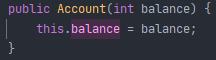
\includegraphics[width=0.7\textwidth]{sources/7_implementering/Account.PNG}
    \caption{Start Beløb}
    \label{fig:chance}
\end{figure}

Derefter kommer metoden "withddraw", som gør det muligt at hæve penge fra spillernes konti. Her er det dog ikke muligt at gå i minus, så ved dette tilfælde sættes spillerens konto til 0:
\begin{figure}[H]
    \centering
    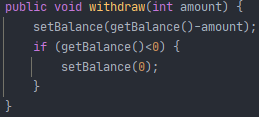
\includegraphics[width=0.7\textwidth]{sources/7_implementering/withdraw.PNG}
    \caption{Metode til at hæve penge}
    \label{fig:chance}
\end{figure}
I denne metode "deposit", kan spillerne moddtage penge. I tilfældet at spilleren konto er i minus, så sættes den til 0 inden beløbet indsættes på kontoen:
\begin{figure}[H]
    \centering
    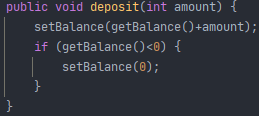
\includegraphics[width=0.7\textwidth]{sources/7_implementering/deposit.PNG}
    \caption{Metode til at indsætte penge}
    \label{fig:chance}
\end{figure}
I metoden "pay", kan spilleren betale husleje til spilleren, som ejer det felt der landes på:
\begin{figure}[H]
    \centering
    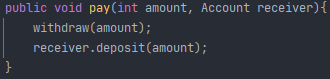
\includegraphics[width=0.7\textwidth]{sources/7_implementering/pay.PNG}
    \caption{Metode til at betale en spiller}
    \label{fig:chance}
\end{figure}
Når et nytspil startes, så tages metoden "getStartingBalance" i brug. Alt afhængigt af antallet af spillere modtager hver spiller et bestemt beløb. Det betyder, at ved 2 spillere, så mådtager hver spiller 20 millioner, ved 3 spiller modtager de hver 13 millioner og ved 4 spillere, modtager de hver 16 millioner. Det beløb den individuelle spiller har kan også kaldes på ved metoden "getBalance":
\begin{figure}[H]
    \centering
    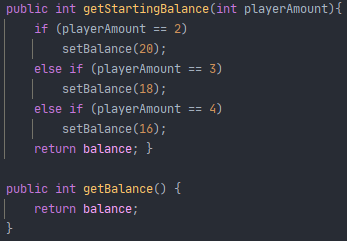
\includegraphics[width=0.7\textwidth]{sources/7_implementering/startBal.PNG}
    \caption{Metode for bestemme startbeløb for spillerne}
    \label{fig:chance}
\end{figure}
Inden spillerne har modtaget et start beløb, så er vi nødt til at definere et beløb til dem. Derfor har de bare 0 millioner, men det har ikke rigtig nongen betydning.
\begin{figure}[H]
    \centering
    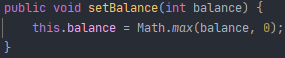
\includegraphics[width=0.7\textwidth]{sources/7_implementering/getBal.png}
    \caption{Midlertidigt startbeløb}
    \label{fig:chance}
\end{figure}
